% Chapter Template

\chapter{Ensayos y resultados} % Main chapter title
En este capítulo se explican las pruebas realizadas al hardware, firmware , controladores y a la plataforma IoT a lo largo del trabajo.
\label{Chapter4} % Change X to a consecutive number; for referencing this chapter elsewhere, use \ref{ChapterX}

%----------------------------------------------------------------------------------------
%	SECTION 1
%----------------------------------------------------------------------------------------

\section{Pruebas unitarias drivers}
Para el desarrollo de los drivers del módulo BG96 y el sensor AHT10 se utilizó la metodología de desarrollo TDD. Esto implica que se escribieron pruebas unitarias para los drivers utilizando ceedling herramienta para el desarrollo de pruebas automáticas. En el código  \ref{cod:codigo test driver AHT10} y \ref{cod:codigo test driver bg96} se pueden ver algunas pruebas unitarias para los drivers desarrollados.
\begin{lstlisting}[label=cod:codigo test driver AHT10,caption=Tests del driver sensor AHT10.]
//Prueba de funcion para obtener el estado del sensor AHT10
void test_estado_del_sensor(void)
{
  uint8_t buffer[1]={0};
  uint8_t data=0;
  read_I2C_STM32L432_port_ExpectAndReturn(AHT10_ADDRESS_SLAVE,buffer,1,AHT10_OK);
  read_I2C_STM32L432_port_ReturnThruPtr_buffer(&data);
  TEST_ASSERT_EQUAL(SENSOR_IDLE,aht10_get_status(&aht10config));
  
  data=255;
  read_I2C_STM32L432_port_ExpectAndReturn(AHT10_ADDRESS_SLAVE,buffer,1,AHT10_OK);
  read_I2C_STM32L432_port_ReturnThruPtr_buffer(&data);
  TEST_ASSERT_EQUAL(SENSOR_BUSY,aht10_get_status(&aht10config));
  
  read_I2C_STM32L432_port_ExpectAndReturn(AHT10_ADDRESS_SLAVE,buffer,1,AHT10_ERROR);
  TEST_ASSERT_EQUAL(SENSOR_BUSY,aht10_get_status(&aht10config)); 
}

//Prueba para la funcion para obtener el valor de la humedad
void test_obtener_humedad(void)
{
  uint8_t bufferRead[6]={0};
  uint8_t humedad=0;
  uint8_t cmd[3] = {AHT10_CMD_TRIGGER_MEASUREMENT,AHT10_CMD_DATO_0,AHT10_CMD_DATO_1};
  uint8_t buffer[1]={0};
  write_I2C_STM32L432_port_ExpectAndReturn(AHT10_ADDRESS_SLAVE,cmd,3,AHT10_OK);
  delay_STM32L432_port_Expect(AHT10_DELAY_LAUNCH_MEASUREMENT);
  read_I2C_STM32L432_port_ExpectAndReturn(AHT10_ADDRESS_SLAVE,buffer,1,AHT10_OK);
  write_I2C_STM32L432_port_ExpectAndReturn(AHT10_ADDRESS_SLAVE,cmd,3,AHT10_OK);
  delay_STM32L432_port_Expect(AHT10_DELAY_LAUNCH_MEASUREMENT); 
  read_I2C_STM32L432_port_ExpectAndReturn(AHT10_ADDRESS_SLAVE,bufferRead,6,AHT10_OK);
  TEST_ASSERT_EQUAL(AHT10_OK,aht10_get_humedity(&aht10config,&humedad));
  TEST_ASSERT_EQUAL(0,humedad);

  write_I2C_STM32L432_port_ExpectAndReturn(AHT10_ADDRESS_SLAVE,cmd,3,AHT10_ERROR);
  TEST_ASSERT_EQUAL(AHT10_ERROR,aht10_get_humedity(&aht10config,&humedad));

  write_I2C_STM32L432_port_ExpectAndReturn(AHT10_ADDRESS_SLAVE,cmd,3,AHT10_OK);
  delay_STM32L432_port_Expect(AHT10_DELAY_LAUNCH_MEASUREMENT);
  read_I2C_STM32L432_port_ExpectAndReturn(AHT10_ADDRESS_SLAVE,buffer,1,AHT10_OK);
  write_I2C_STM32L432_port_ExpectAndReturn(AHT10_ADDRESS_SLAVE,cmd,3,AHT10_OK);
  delay_STM32L432_port_Expect(AHT10_DELAY_LAUNCH_MEASUREMENT); 
  read_I2C_STM32L432_port_ExpectAndReturn(AHT10_ADDRESS_SLAVE,bufferRead,6,AHT10_ERROR);
  TEST_ASSERT_EQUAL(AHT10_ERROR,aht10_get_humedity(&aht10config,&humedad));
}
\end{lstlisting}

\begin{lstlisting}[label=cod:codigo test driver bg96,caption=Tests del driver modulo bg96.] 
//Prueba para la funcion para obtener el estado en el que se encuentra el modulo bg96
void test_get_status_modem(void)
{
  char buffer_resp[20]={0};
  send_data_ExpectAndReturn(CMD_BG96_STATUS_MODEM,RS_BG96_OK,buffer_resp,1000,FT_BG96_OK);
  TEST_ASSERT_EQUAL(FT_BG96_OK,get_status_modem(&config_module));

  send_data_ExpectAndReturn(CMD_BG96_STATUS_MODEM,RS_BG96_OK,buffer_resp,1000,FT_BG96_ERROR);
  TEST_ASSERT_EQUAL(FT_BG96_ERROR,get_status_modem(&config_module));
}

//Prueba de la funcion para mandar sms  
void test_send_sms_bg96(void)
{
  char buffer_resp[30]={0};
  send_data_ExpectAndReturn("AT+CMGS=\"72950576\"\r",RS_BG96_SIGNAL,buffer_resp,12000,FT_BG96_OK);
  send_data_ExpectAndReturn("HOLA\x1a\r",RS_BG96_OK,buffer_resp,12000,FT_BG96_OK);
  TEST_ASSERT_EQUAL(FT_BG96_OK,send_sms_bg96(&config_module,"72950576","HOLA"));

  send_data_ExpectAndReturn("AT+CMGS=\"72950576\"\r",RS_BG96_SIGNAL,buffer_resp,12000,FT_BG96_ERROR);
  TEST_ASSERT_EQUAL(FT_BG96_ERROR,send_sms_bg96(&config_module,"72950576","HOLA"));

  send_data_ExpectAndReturn("AT+CMGS=\"72950576\"\r",RS_BG96_SIGNAL,buffer_resp,12000,FT_BG96_OK);
  send_data_ExpectAndReturn("HOLA\x1a\r",RS_BG96_OK,buffer_resp,12000,FT_BG96_ERROR);
  TEST_ASSERT_EQUAL(FT_BG96_ERROR,send_sms_bg96(&config_module,"72950576","HOLA"));
}

//Prueba de la funcion para publicar mensajes al broker mqtt
void test_publish_message(void)
{
  char buffer_resp[30]={0};
  char topic[19]="/v1.6/devices/demo";
  char data[25]="{\"demo\":10,\"humedad\":60}";
  send_data_ExpectAndReturn("AT+QMTPUB=0,0,0,0,\"/v1.6/devices/demo\"\r",RS_BG96_SIGNAL,buffer_resp,3000,FT_BG96_OK);
  send_data_ExpectAndReturn("{\"demo\":10,\"humedad\":60}\x1a\r",RS_BG96_CERO,buffer_resp,15000,FT_BG96_OK);
  TEST_ASSERT_EQUAL(FT_BG96_OK,publish_message(&config_module,topic,data));

  send_data_ExpectAndReturn("AT+QMTPUB=0,0,0,0,\"/v1.6/devices/demo\"\r",RS_BG96_SIGNAL,buffer_resp,3000,FT_BG96_ERROR);
  TEST_ASSERT_EQUAL(FT_BG96_ERROR,publish_message(&config_module,topic,data));

  send_data_ExpectAndReturn("AT+QMTPUB=0,0,0,0,\"/v1.6/devices/demo\"\r",RS_BG96_SIGNAL,buffer_resp,3000,FT_BG96_OK);
  send_data_ExpectAndReturn("{\"demo\":10,\"humedad\":60}\x1a\r",RS_BG96_CERO,buffer_resp,15000,FT_BG96_ERROR);
  TEST_ASSERT_EQUAL(FT_BG96_ERROR,publish_message(&config_module,topic,data));
}
\end{lstlisting}

Una forma cuantitativa de evaluar estas pruebas son los informes de cobertura generados por ceedling.

En la figura \ref{fig:Cobertura aht10} se puede observar el informe de cobertura del driver aht10, donde se puede apreciar que las pruebas ejecutan el 100\% de las líneas de código escritas y explora el 100\% de las combinaciones en los saltos de condicionales.

En la figura \ref{fig:Cobertura BG96} también se observa el informe de cobertura del driver de bg96, con 98.4\% de líneas ejecutadas y explora más del 98.3\% de combinaciones posibles. 

\begin{figure}[h!]
    \centering
      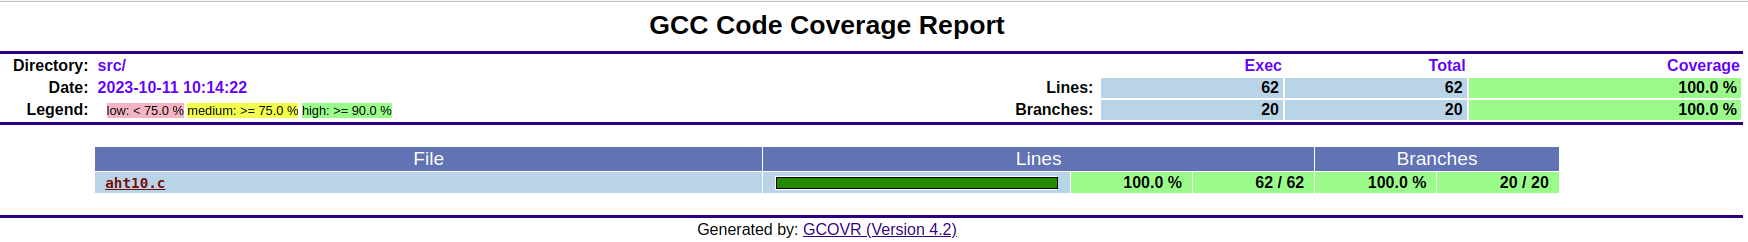
\includegraphics[width=\linewidth, height=6cm]{./Figures/cobertura_aht10.png}
    \caption{Informe de cobertura driver aht10.}
      \label{fig:Cobertura aht10}
  \end{figure}

\begin{figure}[htbp!]
    \centering
      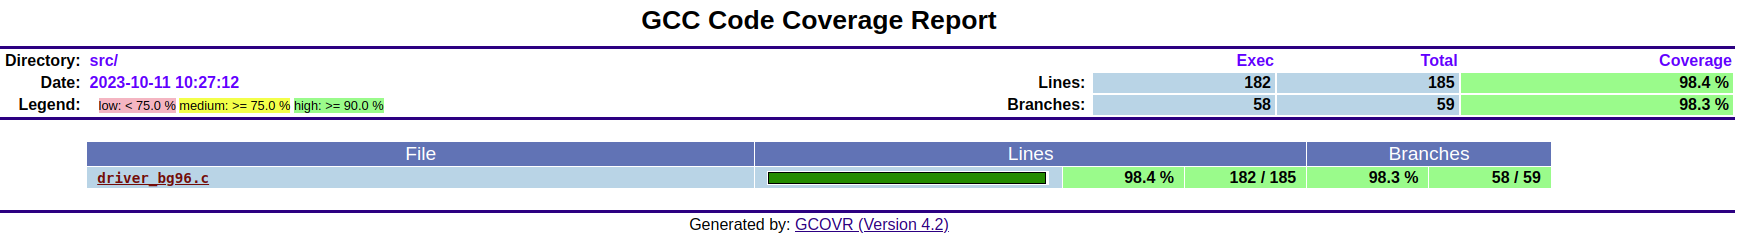
\includegraphics[width=\linewidth, height=6cm]{./Figures/cobertura_bg96.png}
    \caption{Informe de cobertura driver BG96.}
      \label{fig:Cobertura BG96}
\end{figure}

\section{Pruebas de la plataforma IoT}
\subsection{Pruebas de inyeccion de mensajes}
El objetivo de las pruebas de inyección de mensajes a la plataforma IoT es evaluar la llegada de los mensajes por protocolo MQTT al servidor.
Para realizar el envío de datos a broker MQTT, se utiliza el cliente MQTT de mosquitto ejecutando el comando que se muestra en la figura \ref{fig:mosquitto pub}.

\begin{figure}[h!]
  \centering
    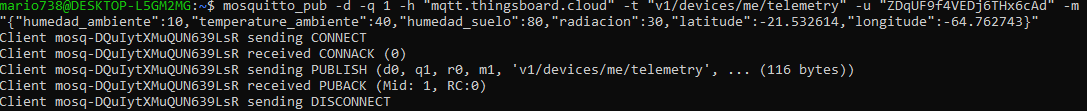
\includegraphics[width=\linewidth, height=3cm]{./Figures/mosquito_enviodatos.png}
  \caption{Envio de datos por el cliente MQTT de mosquitto.}
    \label{fig:mosquitto pub}
\end{figure}

Donde:
\begin{itemize}
  \item -h dirección del broker
  \item -t tópico 
  \item -u token
  \item -m mensaje en formato json
\end{itemize}

Al ejecutar el comando podemos ver que el cliente mqtt primeramente se conecta al broker mqtt luego publica el mensaje en el topico escogido y finalmente se desconecta del servidor.

Para comprobar la llegada de los valores al broker de ThingsBoard tenemos que ir a la sección dispositivos, seleccionar el dispositivo al que se le envio los datos y entrar a la pestaña de última telemetría, en la figura \ref{fig:tb recepcion} podemos ver que los datos llegaron correctamente.

\begin{figure}[h!]
  \centering
    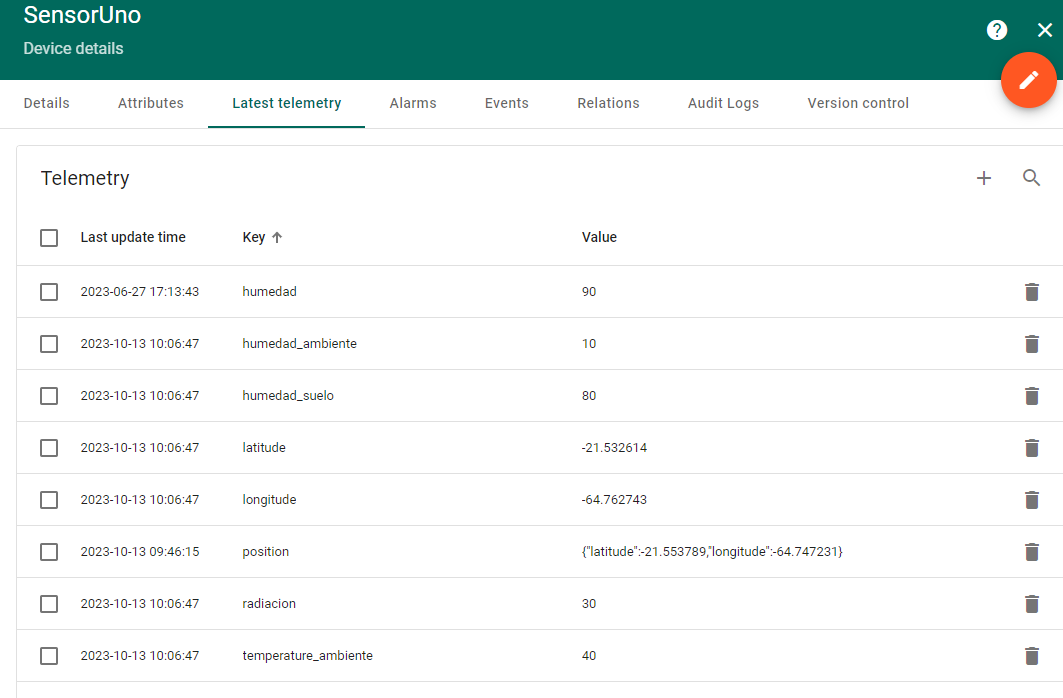
\includegraphics[width=6cm, height=9.5cm]{./Figures/tb_recepcion.png}
  \caption{Recepción de datos en el broker MQTT.}
    \label{fig:tb recepcion}
\end{figure}

\subsection{Prueba de la tabla de alarmas en thingsboard}
La plataforma permite configurar alarmas con respecto a las variables monitoreadas, en el panel de visualización de cada sensor se tiene una tabla de alarmas que muestran las notificaciones de las alarmas que se activaron.
En la figura \ref{fig:alarmas tb} podemos ver la notificación de una alarma cuando la temperatura ambiente del sistema sobrepasa los 43 grados centígrados.

\begin{figure}[h!]
  \centering
    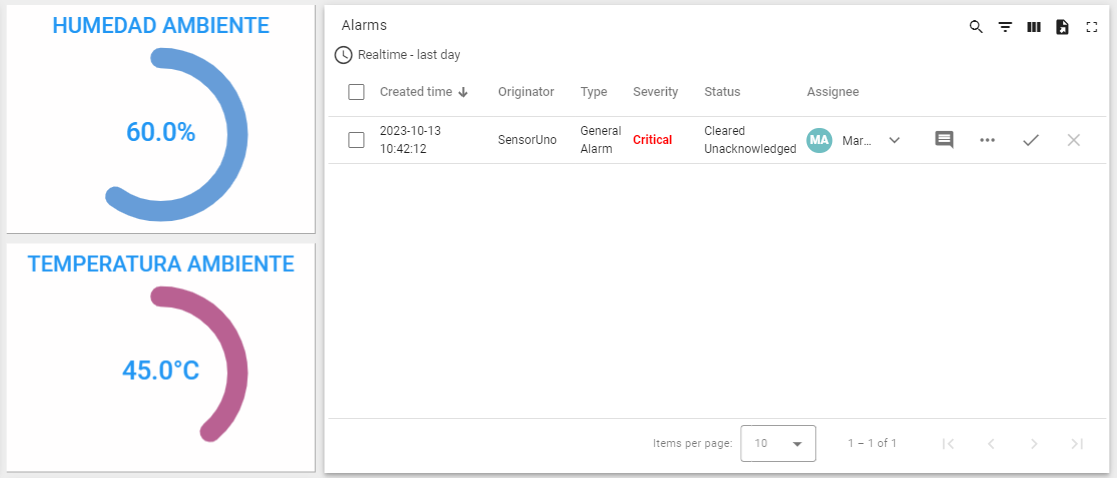
\includegraphics[width=\linewidth, height=7cm]{./Figures/alarmas_tb.png}
  \caption{Tabla de alarmas activas.}
    \label{fig:alarmas tb}
\end{figure}

\subsection{Prueba del widget de mapa}
En los paneles de visualización tenemos mapas con la ubicación del lugar donde se implementó el dispositivo.
En la figura \ref{fig:map thingsboard}  podemos ver la ubicación del sensor implementado para el proyecto.

\begin{figure}[h!]
  \centering
    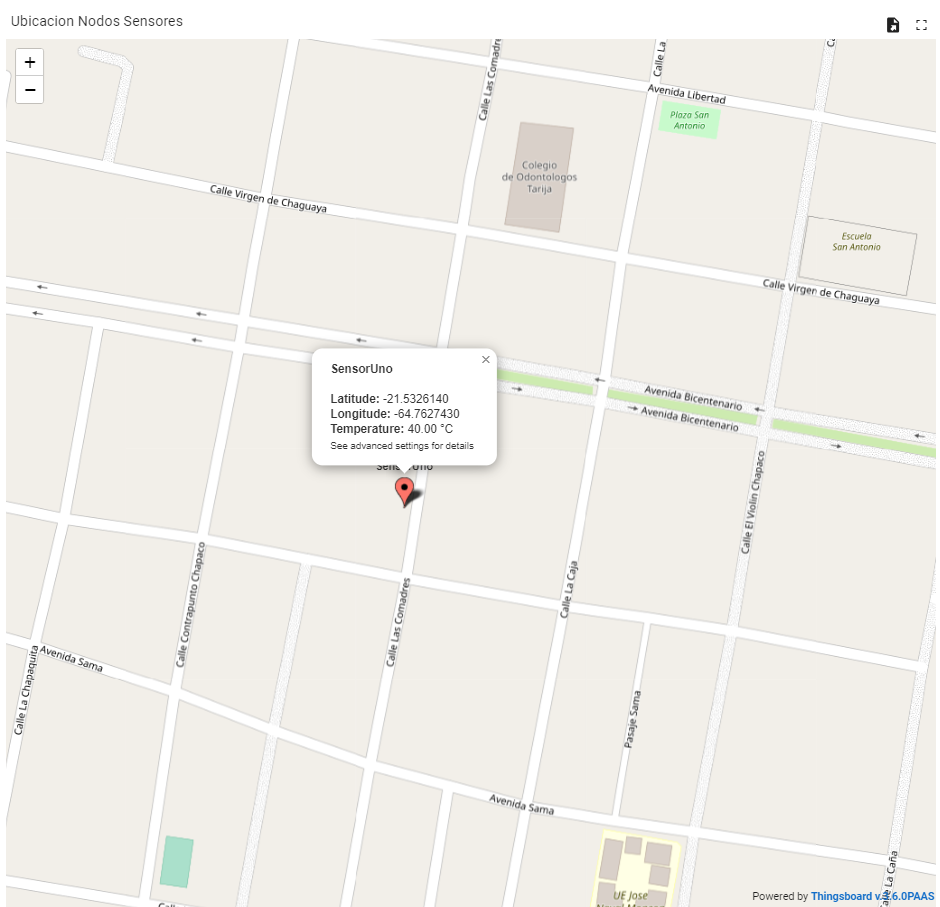
\includegraphics[width=12cm, height=8cm]{./Figures/map.png}
  \caption{Ubicación del nodo sensor implementado.}
    \label{fig:map thingsboard}
\end{figure}

\subsection{Prueba de persistencia de datos}
Para realizar la prueba de persistencia de datos se configuró en el panel de visualización, las gráficas con un entorno de tiempo más amplio.
En las gráficas se estableció un rango de tiempo de 7 días. El resultado se muestra en la figura \ref{fig:Persistencia de datos}.

\begin{figure}[h!]
  \centering
    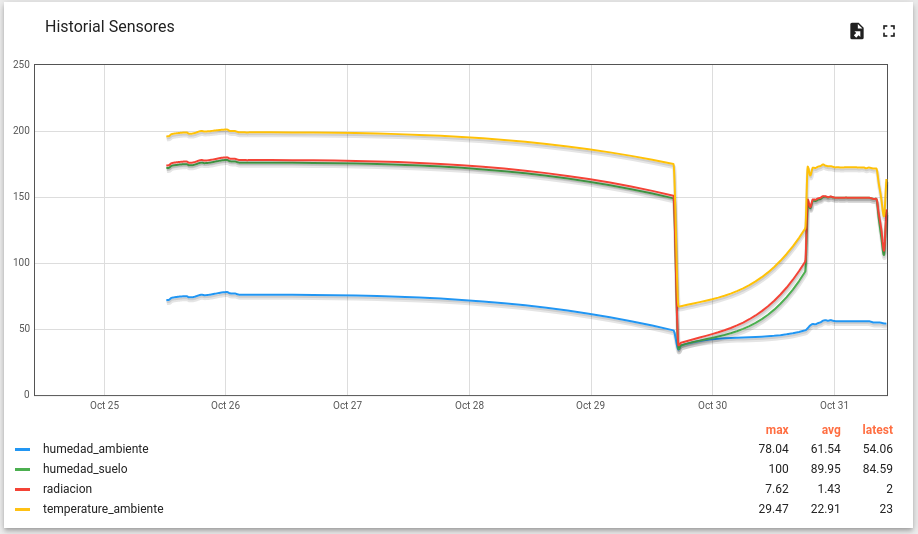
\includegraphics[width=10cm, height=6cm]{./Figures/historial_sensores.png}
  \caption{Persistencia de datos.}
    \label{fig:Persistencia de datos}
\end{figure}

\clearpage 
\section{Pruebas De Hardware}
\subsection{Prueba comunicación sensor de humedad AHT10}
Para probar el correcto funcionamiento del sensor AHT10 y la correcta comunicación con el microcontrolador se comprobó la trama I2C con un analizador lógico,
en la figura \ref{fig:write aht10} podemos ver la trama capturada cuando queremos escribir en un registro del sensor y en la figura \ref{fig:read aht10} tenemos la trama cuando leemos los registros del sensor donde se obtiene 6 bytes en los que se encuentra la información de la humedad y la temperatura.

\begin{figure}[h!]
  \centering
    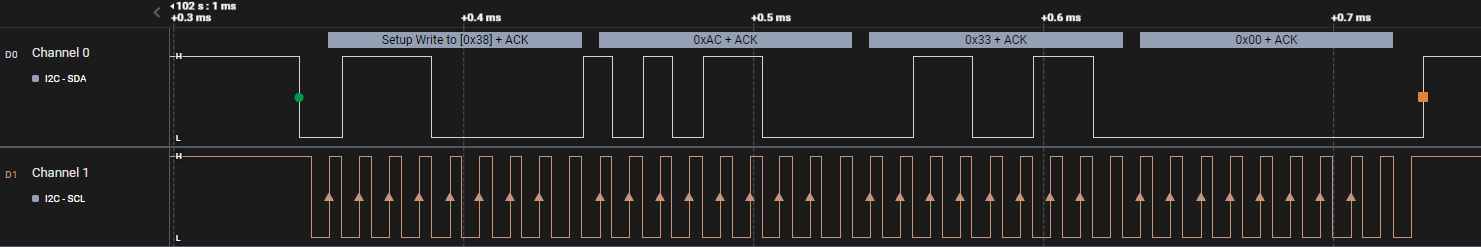
\includegraphics[width=\linewidth, height=3.5cm]{./Figures/write_i2c.png}
  \caption{Trama de escritura al sensor AHT10.}
    \label{fig:write aht10}
\end{figure}

\begin{figure}[h!]
  \centering
    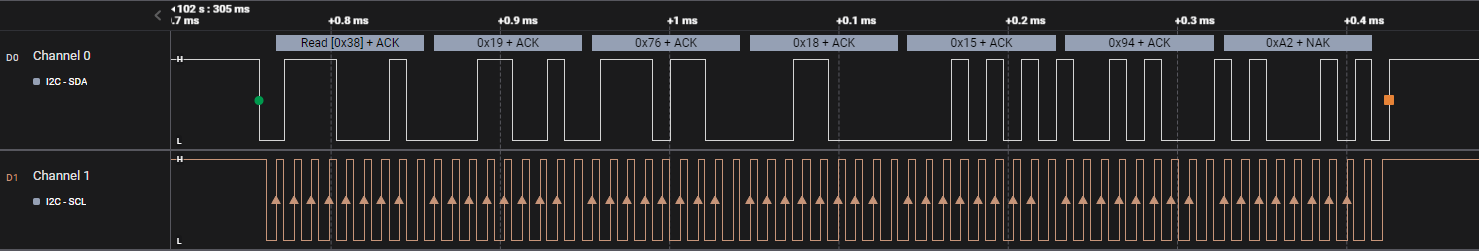
\includegraphics[width=\linewidth, height=3.5cm]{./Figures/read_i2c..png}
  \caption{Trama de lectura del sensor AHT10.}
    \label{fig:read aht10}
\end{figure}

\subsection{Pruebas comunicación modulo BG96}

Para probar la comunicación del microcontrolador con el módulo bg96 se utilizó un analizador lógico que nos permite ver los comandos que envía el microcontrolador y la respuestas del módulo a estos comandos por el puerto UART.
En la figura \ref{fig:trama uart1} vemos dos canales del analizador  lógico el canal 2 muestra un comando mandado por el microcontrolador al módulo de comunicación y en el canal 3 la respuesta del módulo al comando enviado.

\begin{figure}[h!]
  \centering
    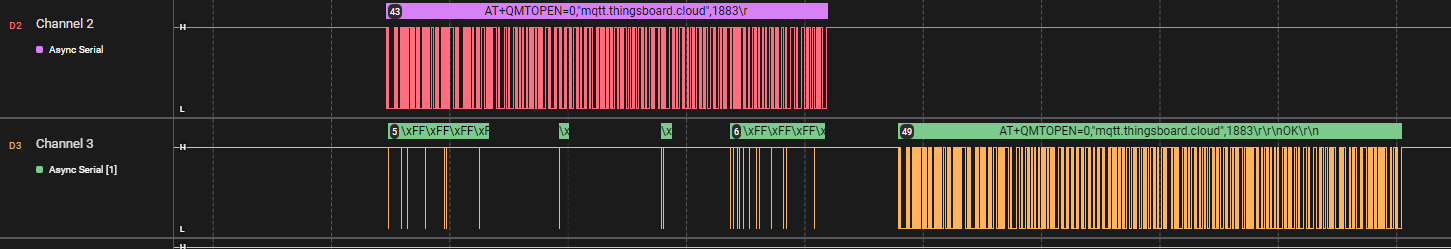
\includegraphics[width=\linewidth, height=3.5cm]{./Figures/trama_uart1.png}
  \caption{Envío y recepción de comandos por puerto UART.}
    \label{fig:trama uart1}
\end{figure}

\subsection{Pruebas de alimentacion }
Se probaron las fuentes de alimentación del sistema, la batería de 12V para el microcontrolador y la batería de 3.7V para el módulo de comunicación bg96.
En la figuras muestran las pruebas de alimentación del sistema.


\subsection{Prueba microcontrolador en bajo consumo }
Al ser un dispositivo que funciona a batería lo que busca el firmware es consumir lo menos posible, por lo tanto el sistema entra en bajo consumo en los momentos en que el microcontrolador no realiza ninguna función. 
En la figura podemos ver el consumo del sistema normalmente y en la figura el consumo bajo consumo.




\clearpage 
\section{Pruebas Funcionales del sistema}
Para realizar las pruebas funcionales de todo el sistema se implementó el dispositivo en un lugar donde se tiene un cultivo de tomate como se muestra en la figura.

\subsection{Prueba de lectura de sensores}
Se realizó la lectura de todos los sensores y se mando los datos obtenidos al servidor mqtt .La figura muestra la lectura de los datos adquiridos.

Las figuras muestran las pruebas que se realizaron a las lecturas del sensor de humedad se suelo en diferentes casos, cuando el suelo está húmedo la lectura del sensor es  45 por ciento y cuando el suelo está seco la lectura del sensor es 10.

La lectura del sensor de radiación es de 3 que significa que la radiación es moderada la lectura en horas del mediodía donde el sol da con más fuerza en el lugar de la implementación.


\subsection{Prueba de envío de datos al broker mqtt}
Una de las tareas más importante del firmware es la del manejo del servidor, para verificar el correcto funcionamiento de esta tarea tenemos que ver la secuencia de comandos que son mandados del microcontrolador al módulo de comunicación por el puerto UART.
Para realizar esta prueba se conectó un convertidor UART a USB al conector de debug que tiene nuestro dispositivo, con este convertidor podemos ver todos los comandos que el microcontrolador manda al módulo de comunicación.
En la figura podemos observar toda la secuencia de comandos que realiza el firmware para realizar el envío de datos a la plataforma IoT, como vemos  primeramente se verifica si el módulo está activo, luego se configura el apn de la red, luego se conecta al broker mqtt , se publican  los datos al servidor y finalmente el realizar el proceso de desconexión.

\begin{figure}[h]
  \centering
    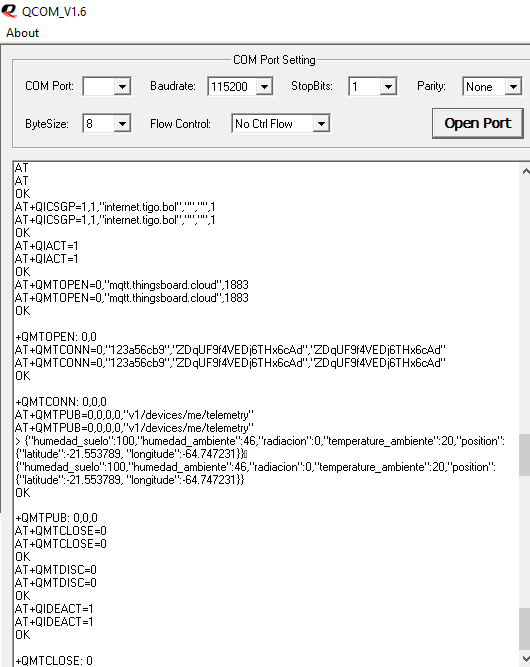
\includegraphics[width=8cm, height=12cm]{./Figures/Qcom_enviodedatos.png}
  \caption{Comandos para enviar datos al broker mqtt.}
    \label{fig:conexion broker}
\end{figure}

\subsection{Pruebas de alarmas}
El objetivo de esta prueba es comprobar el buen funcionamiento de las alarmas del sistema.
Cuando la humedad del suelo baja por debajo del rango permitido por el sistema, el firmware manda un sms al usuario con la alarma ocurrida.En la figura podemos ver que la humedad bajo de 10\% y en la figura se ve que se recibió el sms.

\begin{figure}[h!]
  \centering
    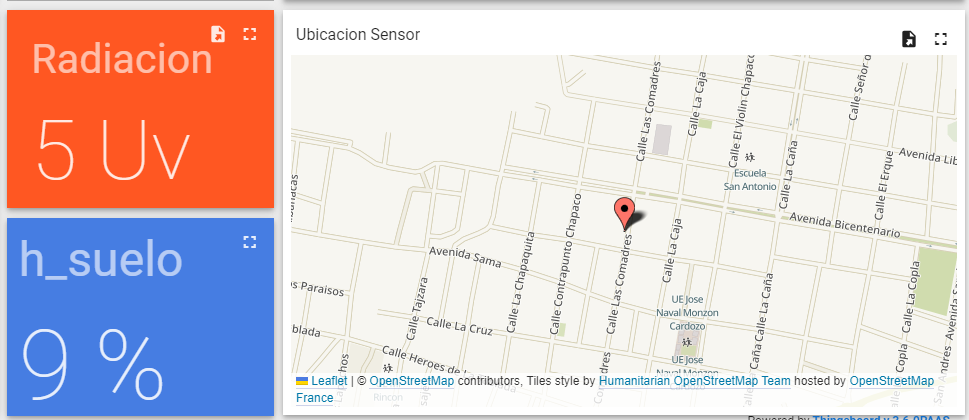
\includegraphics[width=\linewidth, height=7cm]{./Figures/humedad_menor2.png}
  \caption{Informe de cobertura driver aht10.}
    \label{fig:humedad menor}
\end{figure}

\begin{figure}[h!]
  \centering
    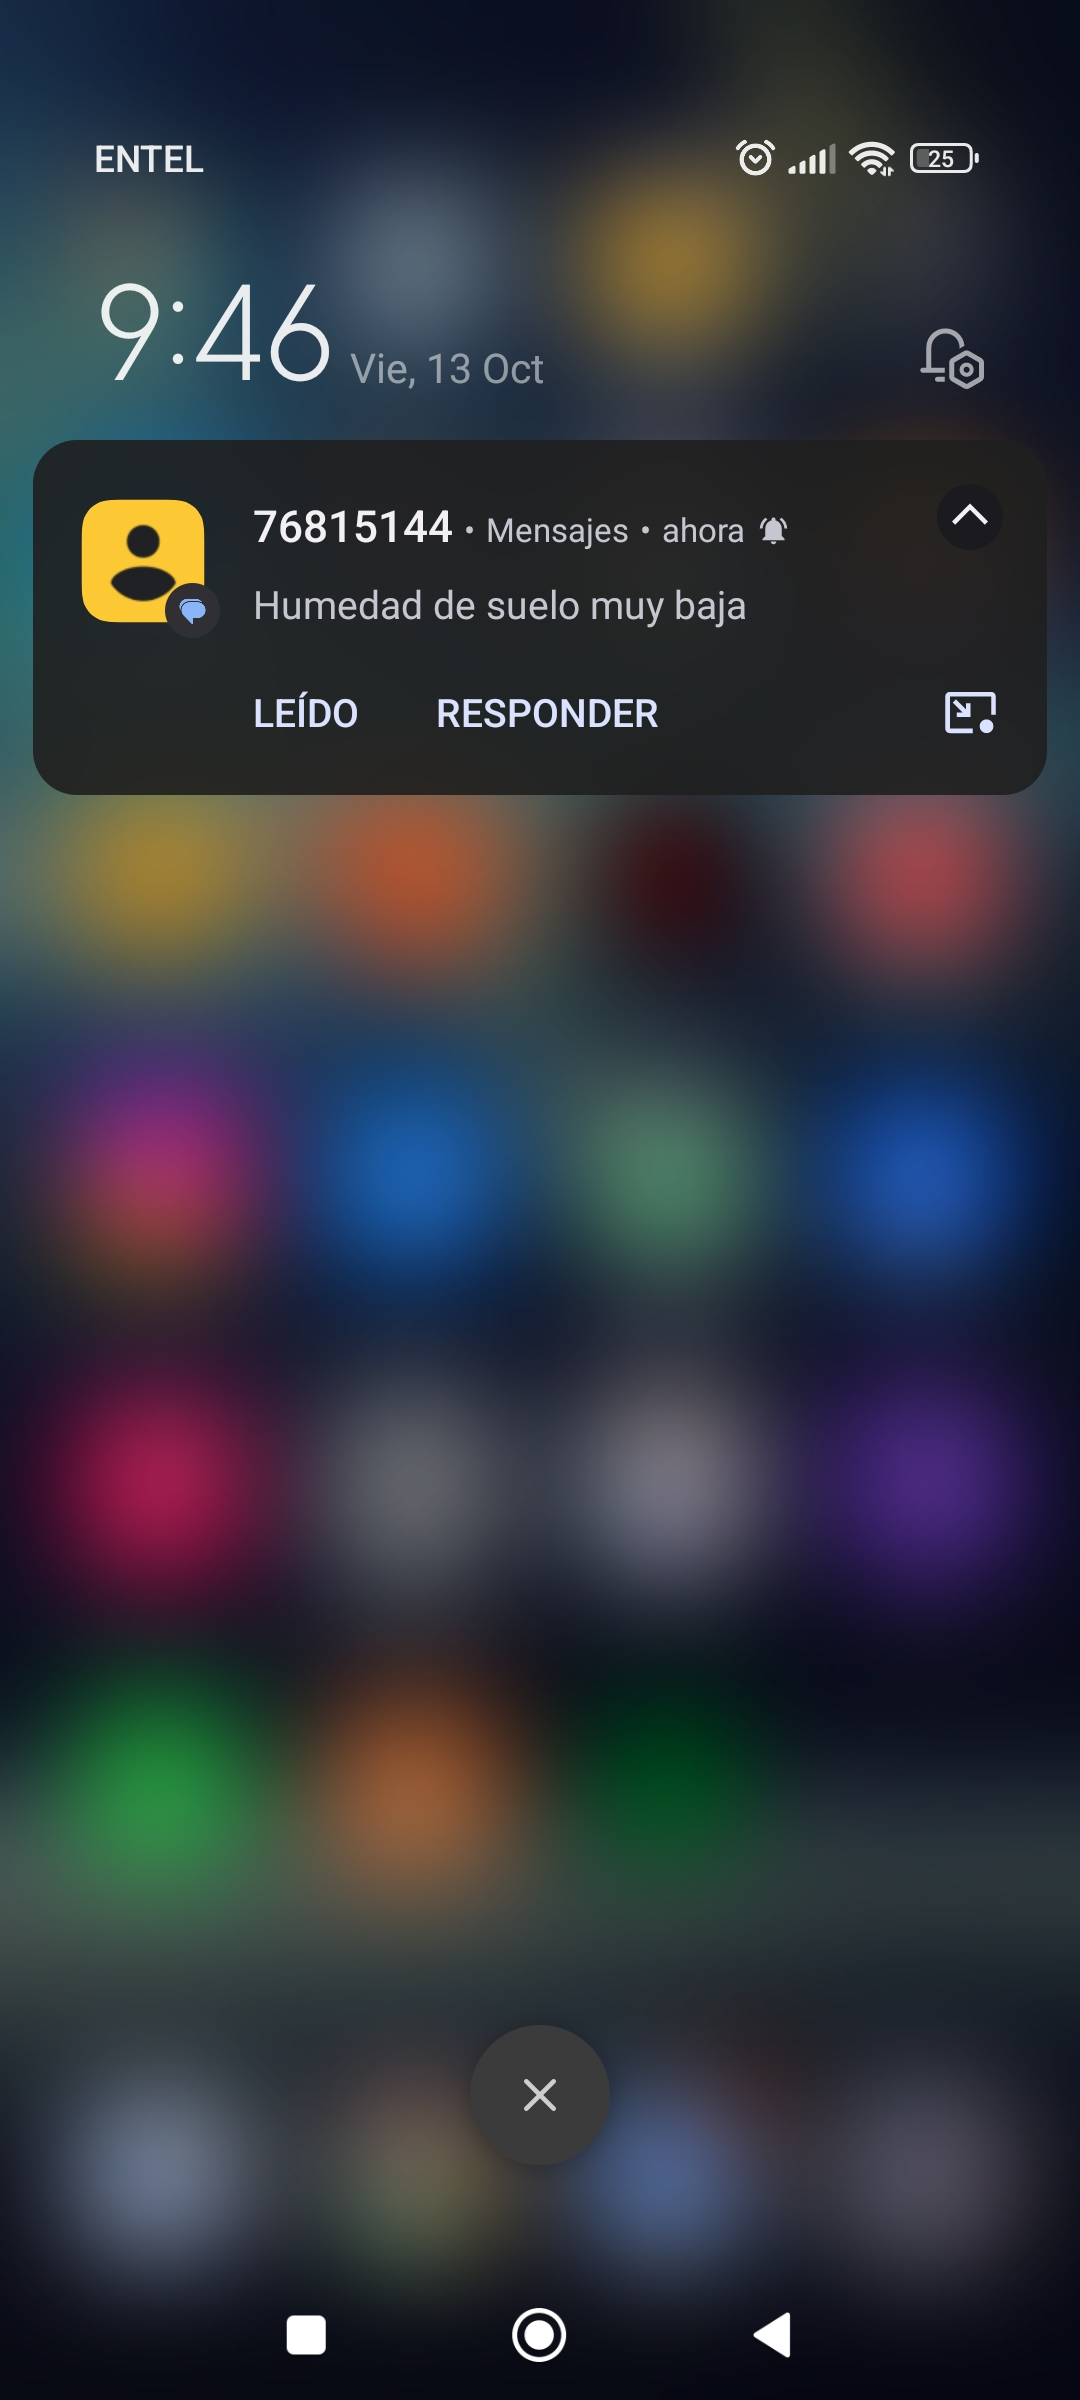
\includegraphics[width=8cm, height=12cm]{./Figures/sms_alarma.jpg}
  \caption{Informe de cobertura driver aht10.}
    \label{fig:sms alarma}
\end{figure}

\label{sec:pruebasHW}

